\documentclass[
	9pt, % Set the default font size, options include: 8pt, 9pt, 10pt, 11pt, 12pt, 14pt, 17pt, 20pt
	t, % Uncomment to vertically align all slide content to the top of the slide, rather than the default centered
	%aspectratio=169, % Uncomment to set the aspect ratio to a 16:9 ratio which matches the aspect ratio of 1080p and 4K screens and projectors
]{beamer}

\graphicspath{{Images/}{./}} % Specifies where to look for included images (trailing slash required)

\usepackage{booktabs} % Allows the use of \toprule, \midrule and \bottomrule for better rules in tables
\usepackage{graphicx}
\usepackage{caption}
\usepackage{subcaption}
\usepackage{hyperref}
\usepackage[english,brazil]{babel}
\usepackage{fontawesome5}
\usepackage{listings}
\usepackage{minted}
\usepackage{xcolor}
% \usepackage{graphicx}
% \usepackage{animate}
\RequirePackage[backend=biber,
style=ieee,
citestyle=authoryear,
]{biblatex}

% Define a custom command for an icon link
\newcommand{\iconLink}[2]{\href{#1}{\faLink \hspace{0.2em} {#2}}}
\newcommand{\yellowbox}[1]{\colorbox{yellow!75}{#1}}
\definecolor{darkgreen}{rgb}{0,0.5,0}

% Definindo um estilo para o destaque
%----------------------------------------------------------------------------------------
%	SELECT LAYOUT THEME
%----------------------------------------------------------------------------------------
\usetheme{Madrid}

%----------------------------------------------------------------------------------------
%	SELECT COLOR THEME
%----------------------------------------------------------------------------------------

% Beamer comes with a number of color themes that can be applied to any layout theme to change its colors. Uncomment each of these in turn to see how they change the colors of your selected layout theme.

%\usecolortheme{albatross}
%\usecolortheme{beaver}
%\usecolortheme{beetle}
% \usecolortheme{crane}
%\usecolortheme{dolphin}
%\usecolortheme{dove}
%\usecolortheme{fly}
%\usecolortheme{lily}
%\usecolortheme{monarca}
%\usecolortheme{seagull}
%\usecolortheme{seahorse}
%\usecolortheme{spruce}
%\usecolortheme{whale}
%\usecolortheme{wolverine}

%----------------------------------------------------------------------------------------
%	SELECT FONT THEME & FONTS
%----------------------------------------------------------------------------------------
\usefonttheme{default} % Typeset using the default sans serif font

%------------------------------------------------

\usepackage{palatino} % Use the Palatino font for serif text
\usepackage[default]{lato} % Use the Lato font for sans serif text

%----------------------------------------------------------------------------------------
%	SELECT INNER THEME
%----------------------------------------------------------------------------------------
\useinnertheme{rectangles}

%----------------------------------------------------------------------------------------
%	SELECT OUTER THEME
%----------------------------------------------------------------------------------------

% Outer themes change the overall layout of slides, such as: header and footer lines, sidebars and slide titles. Uncomment each theme in turn to see what changes it makes to your presentation.

%\useoutertheme{default}
%\useoutertheme{infolines}
%\useoutertheme{miniframes}
%\useoutertheme{smoothbars}
%\useoutertheme{sidebar}
%\useoutertheme{split}
%\useoutertheme{shadow}
%\useoutertheme{tree}
%\useoutertheme{smoothtree}

%\setbeamertemplate{footline} % Uncomment this line to remove the footer line in all slides
%\setbeamertemplate{footline}[page number] % Uncomment this line to replace the footer line in all slides with a simple slide count

%\setbeamertemplate{navigation symbols}{} % Uncomment this line to remove the navigation symbols from the bottom of all slides

% \bibliography{references} % Specifies the bibliography file to include publications
% \bibliographystyle{apalike} % Specifies the bibliography style
\addbibresource{references.bib}

%----------------------------------------------------------------------------------------
%	PRESENTATION INFORMATION
%----------------------------------------------------------------------------------------

\title[DesWebII]{Desenvolvimento Web II} % The short title in the optional parameter appears at the bottom of every slide, the full title in the main parameter is only on the title page
\subtitle{Aula 10 - HTTP/2} % Presentation subtitle, remove this command if a subtitle isn't required
\author[Fabricio Bizotto]{Prof. Fabricio Bizotto} % Presenter name(s), the optional parameter can contain a shortened version to appear on the bottom of every slide, while the main parameter will appear on the title slide
\institute[IFC]{Instituto Federal Catarinense \\ \smallskip \textit{fabricio.bizotto@ifc.edu.br}} % Your institution, the optional parameter can be used for the institution shorthand and will appear on the bottom of every slide after author names, while the required parameter is used on the title slide and can include your email address or additional information on separate lines
\date[\today]{Ciência da Computação \\ \today} % Presentation date or conference/meeting name, the optional parameter can contain a shortened version to appear on the bottom of every slide, while the required parameter value is output to the title slide

%----------------------------------------------------------------------------------------
\begin{document}

%----------------------------------------------------------------------------------------
%	TITLE SLIDE
%----------------------------------------------------------------------------------------

\begin{frame}
	\titlepage % Output the title slide, automatically created using the text entered in the PRESENTATION INFORMATION block above
\end{frame}

%----------------------------------------------------------------------------------------
%	TABLE OF CONTENTS SLIDE
%----------------------------------------------------------------------------------------

\begin{frame}
	\frametitle{Roteiro} % Slide title, remove this command for no title
	
	\tableofcontents % Output the table of contents (all sections on one slide)
	%\tableofcontents[pausesections] % Output the table of contents (break sections up across separate slides)
\end{frame}

%----------------------------------------------------------------------------------------
%	PRESENTATION BODY SLIDES
%----------------------------------------------------------------------------------------

\section{HTTP/2}

\begin{frame}
	\begin{center}
		
		\bigskip\bigskip\bigskip\bigskip % Vertical whitespace
		{\Large HTTP/2}
		
		\bigskip\bigskip % Vertical whitespace
		{\Huge Quais são as principais novidades?}

		\bigskip\bigskip % Vertical whitespace
		{\small Em breve, HTTP/3}
	\end{center}

\end{frame}

\section{Definição}

\begin{frame}
	\frametitle{HTTP/2}
	\framesubtitle{Definição}

	\begin{itemize}
		\item HTTP/2 é a segunda versão do protocolo HTTP.
		\item Foi publicado em 2015.
		\item Objetivo: melhorar a performance do protocolo.
		\item Baseado no protocolo SPDY, desenvolvido pelo Google.
		\item É binário, ao contrário do HTTP/1.1 que é textual.
		\item Principais novidades:
		\begin{itemize}
			\item Multiplexação
			\item Compressão de cabeçalhos
			\item Server Push
			\item Priorização de requisições
		\end{itemize}
	\end{itemize}

\end{frame}

\section{HTTP/2: Multiplexação}

\begin{frame}
	\frametitle{HTTP/2}
	\framesubtitle{Multiplexação}

	\begin{figure}
		\centering
		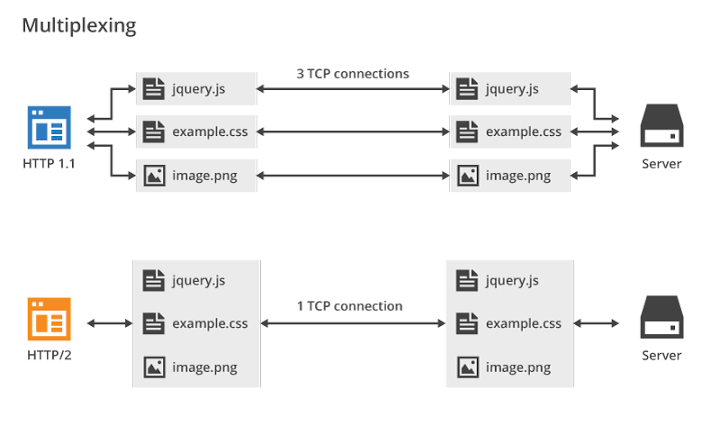
\includegraphics[width=0.9\linewidth]{http_2_multiplexing.png}
		\caption{Multiplexação de requisições no HTTP/2.}
	\end{figure}

\end{frame}

\section{HTTP/2: Compressão de cabeçalhos}

\begin{frame}
	\frametitle{HTTP/2}
	\framesubtitle{Compressão de cabeçalhos}

	\begin{itemize}
		\item HTTP/1.1 precisa criar uma nova requisição para cada recurso.
		\item HTTP/2 pode enviar todos os recursos em uma única conexão, usando compressão de cabeçalhos.
		\item HTTP/1 usa \textbf{gzip}. É utilizado para compressão do corpo da mensagem em respostas HTTP.
		\item HTTP/2 usa \textbf{HPACK}. É utilizado para compressão de cabeçalhos HTTP.
		\item HPACK é um algoritmo de compressão de cabeçalhos baseado em Huffman\footnote{\href{https://kristijansedlak.medium.com/hpack-huffman-encoder-explained-61102edd6ecc}{https://kristijansedlak.medium.com/hpack-huffman-encoder-explained-61102edd6ecc}}.
	\end{itemize}

\end{frame}

\section{HTTP/2: Server Push}

\begin{frame}
	\frametitle{HTTP/2}
	\framesubtitle{Server Push}

	\begin{itemize}
		\item Server Push é uma funcionalidade do HTTP/2 que permite ao servidor enviar recursos para o cliente antes que ele solicite.
		\item O servidor pode enviar recursos que ele acredita que o cliente irá solicitar.
		\item O cliente pode aceitar ou rejeitar os recursos enviados pelo servidor.
		\item Server Push é uma funcionalidade \textbf{opcional}.
	\end{itemize}

	\begin{figure}
		\centering
		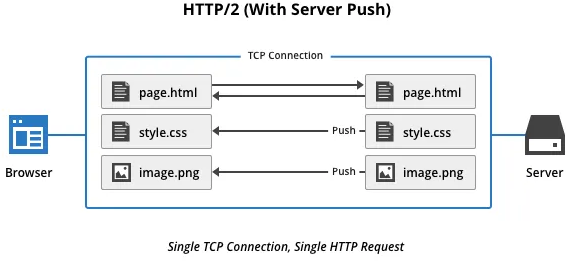
\includegraphics[width=0.7\linewidth]{http2_server_push.png}
		\caption{Server Push no HTTP/2.}
	\end{figure}

\end{frame}

\section{HTTP/2: Priorização de requisições}

\begin{frame}
	\frametitle{HTTP/2}
	\framesubtitle{Priorização de requisições}

	\begin{itemize}
		\item HTTP/2 permite que o cliente priorize as requisições.
		\item O cliente pode informar ao servidor quais requisições são mais importantes.
		\item O servidor pode usar essa informação para priorizar o envio de recursos.
		\item A priorização é feita através de um \textbf{peso} e um \textbf{dependência}.
	\end{itemize}

	\begin{figure}
		\centering
		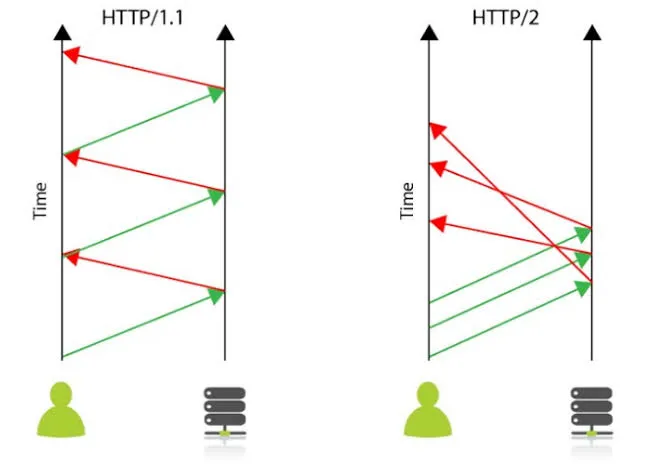
\includegraphics[width=0.7\linewidth]{http2_priority.png}
		\caption{Priorização de requisições no HTTP/2.}
	\end{figure}

\end{frame}

\section{Exemplo}

\begin{frame}
	\begin{center}
		
		\bigskip\bigskip\bigskip\bigskip % Vertical whitespace
		{\Large HTTP/2}
		
		\bigskip\bigskip % Vertical whitespace
		{\Huge Exemplo prático}

		\bigskip\bigskip % Vertical whitespace
		{\small \iconLink{https://gist.github.com/fabricioifc/347d275a65f1ba3371eb854f78d052ec}{Python + Flask + hypercorn}}
	\end{center}

\end{frame}

\section{QUIZ}

\begin{frame}
	\frametitle{QUIZ}
	\framesubtitle{Questão 1/5}

	{\Large Qual é o principal objetivo do protocolo HTTP/2? }

	\begin{exampleblock}{Resposta}
		\begin{enumerate}[a]
			\item Reduzir a complexidade do HTTP/1.1
			\item Melhorar a segurança das comunicações na web
			\item Aumentar a eficiência no carregamento de páginas web
			\item Adicionar mais funcionalidades aos servidores web
		\end{enumerate}
	\end{exampleblock}

\end{frame}

\begin{frame}
	\frametitle{QUIZ}
	\framesubtitle{Questão 1/5}

	{\Large Qual é o principal objetivo do protocolo HTTP/2? }

	\begin{exampleblock}{Resposta}
		\begin{enumerate}[a]
			\item Reduzir a complexidade do HTTP/1.1
			\item Melhorar a segurança das comunicações na web
			\item \textcolor{darkgreen}{Aumentar a eficiência no carregamento de páginas web}
			\item Adicionar mais funcionalidades aos servidores web
		\end{enumerate}
	\end{exampleblock}

\end{frame}

\begin{frame}
	\frametitle{QUIZ}
	\framesubtitle{Questão 2/5}

	{\Large O HTTP/2 utiliza um novo formato de compressão de cabeçalhos. Qual é o nome deste formato? }

	\begin{exampleblock}{Resposta}
		\begin{enumerate}[a]
			\item GZIP
			\item HPACK
			\item Brotli
			\item Deflate
		\end{enumerate}
	\end{exampleblock}

\end{frame}

\begin{frame}
	\frametitle{QUIZ}
	\framesubtitle{Questão 2/5}

	{\Large O HTTP/2 utiliza um novo formato de compressão de cabeçalhos. Qual é o nome deste formato? }

	\begin{exampleblock}{Resposta}
		\begin{enumerate}[a]
			\item GZIP
			\item \textcolor{darkgreen}{HPACK}
			\item Brotli
			\item Deflate
		\end{enumerate}
	\end{exampleblock}

\end{frame}


\begin{frame}
	\frametitle{QUIZ}
	\framesubtitle{Questão 3/5}

	{\Large Quais são algumas das principais características do HTTP/2?	}

	\begin{exampleblock}{Resposta}
		\begin{enumerate}[a]
			\item Multiplexação, Priorização e Compressão de Cabeçalhos
			\item Roteamento, Criptografia e Autenticação
			\item Redirecionamento, Fragmentação e Cache
			\item Assinatura Digital, Segurança de Transporte e Sessões Persistentes
		\end{enumerate}
	\end{exampleblock}

\end{frame}

\begin{frame}
	\frametitle{QUIZ}
	\framesubtitle{Questão 3/5}

	{\Large Quais são algumas das principais características do HTTP/2?	}

	\begin{exampleblock}{Resposta}
		\begin{enumerate}[a]
			\item \textcolor{darkgreen}{Multiplexação, Priorização e Compressão de Cabeçalhos}
			\item Roteamento, Criptografia e Autenticação
			\item Redirecionamento, Fragmentação e Cache
			\item Assinatura Digital, Segurança de Transporte e Sessões Persistentes
		\end{enumerate}
	\end{exampleblock}

\end{frame}

\begin{frame}
	\frametitle{QUIZ}
	\framesubtitle{Questão 4/5}

	{\Large O HTTP/2 introduziu um conceito que permite que o servidor envie ativamente recursos para o cliente antes mesmo de serem solicitados. Qual é esse conceito?	}

	\begin{exampleblock}{Resposta}
		\begin{enumerate}[a]
			\item Server Push
			\item Requisições Antecipadas
			\item Respostas Pró-ativas
			\item Inicialização Rápida
		\end{enumerate}
	\end{exampleblock}

\end{frame}

\begin{frame}
	\frametitle{QUIZ}
	\framesubtitle{Questão 4/5}

	{\Large O HTTP/2 introduziu um conceito que permite que o servidor envie ativamente recursos para o cliente antes mesmo de serem solicitados. Qual é esse conceito?	}

	\begin{exampleblock}{Resposta}
		\begin{enumerate}[a]
			\item \textcolor{darkgreen}{Server Push}
			\item Requisições Antecipadas
			\item Respostas Pró-ativas
			\item Inicialização Rápida
		\end{enumerate}
	\end{exampleblock}

\end{frame}

\begin{frame}
	\frametitle{QUIZ}
	\framesubtitle{Questão 5/5}

	{\Large Em que situações é especialmente benéfico utilizar o HTTP/2? }

	\begin{exampleblock}{Resposta}
		\begin{enumerate}[a]
			\item Em aplicações web com requisitos mínimos de segurança
			\item Em ambientes com largura de banda limitada e conexões instáveis
			\item Em aplicações onde o suporte a WebSockets é essencial
			\item Em páginas web dinâmicas com muitos recursos a serem carregados
		\end{enumerate}
	\end{exampleblock}

\end{frame}

\begin{frame}
	\frametitle{QUIZ}
	\framesubtitle{Questão 5/5}

	{\Large Em que situações é especialmente benéfico utilizar o HTTP/2? }

	\begin{exampleblock}{Resposta}
		\begin{enumerate}[a]
			\item Em aplicações web com requisitos mínimos de segurança
			\item Em ambientes com largura de banda limitada e conexões instáveis
			\item Em aplicações onde o suporte a WebSockets é essencial
			\item \textcolor{darkgreen}{Em páginas web dinâmicas com muitos recursos a serem carregados}
		\end{enumerate}
	\end{exampleblock}

\end{frame}

\begin{frame}
	\frametitle{QUIZ}
	\framesubtitle{Questão 6/5}

	{\Large O HTTP/2 é retrocompatível com o HTTP/1.1. O que isso significa? }

	\begin{exampleblock}{Resposta}
		\begin{enumerate}[a]
			\item Aplicações HTTP/1.1 não podem ser executadas em servidores HTTP/2
			\item Aplicações HTTP/2 não podem acessar recursos servidos por servidores HTTP/1.1
			\item Aplicações HTTP/1.1 podem continuar funcionando normalmente em um ambiente HTTP/2
			\item Aplicações HTTP/2 precisam ser reescritas para serem executadas em ambientes HTTP/1.1
		\end{enumerate}
	\end{exampleblock}

\end{frame}

\begin{frame}
	\frametitle{QUIZ}
	\framesubtitle{Questão 6/5}

	{\Large O HTTP/2 é retrocompatível com o HTTP/1.1. O que isso significa? }

	\begin{exampleblock}{Resposta}
		\begin{enumerate}[a]
			\item Aplicações HTTP/1.1 não podem ser executadas em servidores HTTP/2
			\item Aplicações HTTP/2 não podem acessar recursos servidos por servidores HTTP/1.1
			\item \textcolor{darkgreen}{Aplicações HTTP/1.1 podem continuar funcionando normalmente em um ambiente HTTP/2}
			\item Aplicações HTTP/2 precisam ser reescritas para serem executadas em ambientes HTTP/1.1
		\end{enumerate}
	\end{exampleblock}

\end{frame}

\section{Lista de Exercícios}

\begin{frame}
	\frametitle{Lista de Exercícios}
	\framesubtitle{HTTP/2}

	\begin{enumerate}
		\item Quais são as principais diferenças entre o HTTP/1.1 e o HTTP/2?
		\item Quais são as principais vantagens do HTTP/2 em relação ao HTTP/1.1?
		\item Quais são as principais desvantagens do HTTP/2 em relação ao HTTP/1.1?
		\item O que são e como funcionam os "cabeçalhos de push" no HTTP/2? Dê um exemplo de situação em que eles podem ser úteis.
		\item Sobre HTTP/3. Quais são as principais diferenças em relação ao HTTP/2?
	\end{enumerate}

	\begin{exampleblock}{Entrega}
		\begin{itemize}
			\item Até a próxima aula.
			\item Manuscrito.
		\end{itemize}
	\end{exampleblock}

	\begin{block}{Desafio}
		Implementar um servidor HTTP/2 usando um servidor web (NGinx, Apache, etc.).
	\end{block}

\end{frame}



\end{document} 
